\chapter{JDart et exécution concolique}
	\paragraph{}
		L'idée générale est de rendre la tâche de tester des Applets Java Card moins penible et plus la plus efficace possible.
		Pour cela nous optons pour l'utilisation de l'exécution concolique comme une technique d'analyse, ce qui permet de rendre 
		le système à tester moins obscur et plus prédictible. Surtout quand on est face à des systèmes complexes
		nécessitant des méthodes plus avancées qu'un simple test unitaire.
    
	\paragraph{}
		\textbf{JDart \footnote{JDart : https://github.com/psycopaths/jdart}} est un outil qui permet d'utiliser l'exécution concolique
		comme une technique de tests pour les applications Java.
		\newline
		Il se présente sous forme d'une extension de \gls{JPF} un outil créé par la NASA afin de tester ses applications, y compris les programmes executés sur ses robots astromobiles.
	\section{Exploration des chemins et l'exécution concolique}
		\subsection{Java Path Finder: Exploration des chemins}
			\nocite{JPF}
			
			\paragraph{}
				\gls{JPF} est un outil de vérification des modèles d'états pour le bytecode Java,
				en réalité \gls{JPF} est une \gls{VM} qui exécute le programme donné en entrée autant de fois que nécessaire
				afin d'explorer chaque chemin qu'il contient.
				
				Tout au long de ce processus, \gls{JPF} collecte les anomalies rencontrées telles que l'interblocage des threads et les exceptions non traitées, puis il génére un rapport contenant les traces qui ménent à ces anomalies.
	
			\begin{figure}[H]
				\centering
					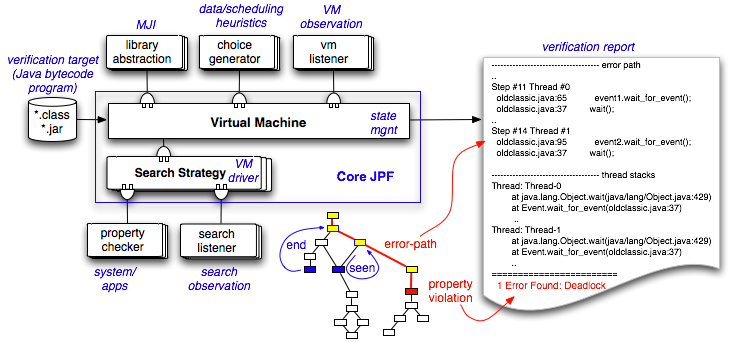
\includegraphics[scale=0.5]{images/jpf-model.png}
				\caption{Modèle d'opération de \gls{JPF}}
			\end{figure}
	
			\paragraph{}
				\gls{JPF} ne se limite pas simplement à détecter les erreurs d'un programme, en effet, il effectue la vérification des modéles.
				C'est un outil qui permet de simuler le non-determinisme. Certains aspects ne peuvent pas être contrôlés par de simples tests et exigent l'assistance d'une \gls{VM}.
				Cependant, en essayant d'explorer et exécuter tous les chemins au sein d'un programme, le nombre d'executions nécessaires peut croître d'une maniére exponentielle (On parle du problème d'explosion d'état). 
				Pour résoudre ce problème, \gls{JPF} réalise une correspondance d'état, c'est un mecanisme qui permet de comparer
				l'état actuel en un n\oe{}ud à des états déjà connus, dans le cas où l'état
				a été verifié \gls{JPF} est capable d'effectuer un retour arrière à la position précédente la plus proche où un chemin inexploré existe et restaure l'état du programme à tester à cette position.
	
			\begin{figure}[H]
				\centering
					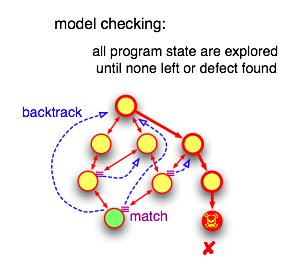
\includegraphics[scale=0.5]{images/jpf-model-checking.png}
				\caption{Vérification du modéles}
			\end{figure}
      
			\paragraph{}
				La vérification des modèles (\textit{Model Checking}) ne dépend pas des conjectures. En théorie si une anomalie est présente dans le programme à tester
				alors la vérification des modéles la trouvera, puisque c'est une méthode qui explore de maniére exhaustive tous les comportements possibles du système ;
				d'où vient l'efficacité du \textit{Model Checking}.
		\subsection{JDart: Exécution concolique}
			\nocite{JDart}
			\nocite{JDart2}

			\paragraph{}
				\gls{JPF} n'est pas une boite noire. L'une des meilleures fonctionalités de \gls{JPF} est la possibilité de le personnaliser entièrement et d'ainsi pouvoir ajouter des extensions facilement.
				Cet aspect a permis la création d'un grand nombre d'extensions utiles comme des moteurs
				qui permettent l'exécution symbolique et concolique.

			\paragraph{}
				Une exécution concolique commence par une entrée concrète, en exécutant le programme à tester, des contraintes symboliques pour les chemins explorés
				sont formés pour cette exécution. Ces contraintes symboliques sont en réalité des formules logiques composées d'un tas de déclarations conditionnelles
				qui ont été collectées tout au long du parcours.

				L'étape suivante consiste à nier une sous formule et donc nous arrivons à créer un nouveau vecteur de valeurs concrétes en utilisant un
				solveur de contraintes.

				Ce vecteur sera utilisé pour une nouvelle exécution du programme ce qui permettra d'éxplorer un nouveau chemin.
				Cette procédure peut être répétée jusqu'à ce que tous les chemins possibles du système à tester soient explorés.
				
			\begin{figure}[H]
				\centering
					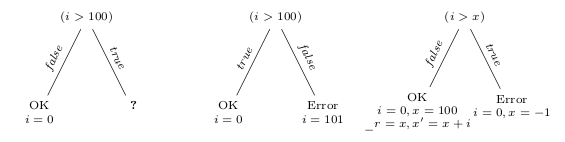
\includegraphics[scale=0.5]{images/concolic.png}
				\caption{Exécution concolique}
			\end{figure}
				
			\paragraph{}
				L'exécution concolique résout un grand problème qui se déclanche généralement au cours de l'exécution concolique, %%Là, je pense qu'il y a une exécution concolique de trop !!!
				puisque l'espace de recherche est réduit significativement de façon à ce que le problème d'explosion d'espace de recherche
				ne peut plus se réaliser car les formules logiques générées par l'execution symbolique indiquera quelle valeur concrète
				doit être fournie pour satisfaire la condition concernée.
				Il n'est plus obligatoire de fournir un grand nombre d'entrées qui, au final, peuvent toutes générer un même chemin.
				\newline
				La technique d'exécution concolique a aussi son effet sur l'exécution symbolique traditionnelle.
				En effet, quand une condition ne peut pas être résolue symboliquement à cause de la complexité de la contrainte (Equation mathématique complexe,
				opération sur les nombres flottant...) elle sera remplacée par une valeur concréte, ce qui permet de continuer l'exploration des chemins.

			\paragraph{}
				JDart est l'une des extensions de \gls{JPF}, il s'agit d'un moteur d'exécution concolique qui traite un programme Java
				en utilisant à la fois des valeurs symboliques et concrétes et garde les traces des exécution symboliques.
				Les formules logiques créées sont ensuite passées à un solveur \textit{\gls{SMT}} afin d'obtenir une évaluation satisfaisante de la contrainte.
				JDart utilise par défaut \textit{\gls{microsoft-z3}} mais  il propose aussi un niveau d'abstraction qui permet d'intégrer d'autres solveurs
				tels que : \textit{Coral} ou \textit{dreal} si nécessaire.
				
			\begin{figure}[H]
				\centering
					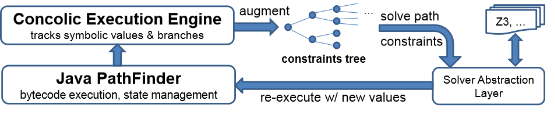
\includegraphics[scale=0.5]{images/archJDart.png}
				\caption{Architecture de JDart}
			\end{figure}
				
			\paragraph{}
				Plus concrètement, la figure~\ref{fig:jdart_sample} montre le résultat d'une portion de code Java executé avec JDart.
				La portion de code admet deux paramétres primitifs et deux simples tests sur ces paramétres, ainsi que la sortie correspondante
				de JDart.
				
			\begin{figure}[H]
				\centering
					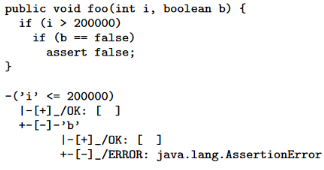
\includegraphics[scale=0.5]{images/jdart_exemple.png}
				\caption{\label{fig:jdart_sample} Exemple d'un programme executé avec JDart}
			\end{figure}
			
			\paragraph{}
				L'arbre des contraintes contient un n\oe{}ud pour chaque condition dans ce fragment de code et deux feuilles.
				Le chemin qui abouti à une erreur est marqué par la classe qui le déclanche.
				Nous n'avons pas affiché les valeurs concrétes qui permettent de parcourir ces chemins, néanmoins, JDart peut être configuré
				de façon à ce qu'il affiche ces valeurs ou génère des tests unitaires basés sur ces valeurs.
      
	\section{La VM JAVA, la VM du JPF et la VM JavaCard}
		\paragraph{}
			Nous avons défini \gls{JPF} comme étant une machine virtuelle qui exécute un code Java et analyse son \textit{\gls{bytecode}},
			Pour pouvoir exécuter le programme à tester, la machine virtuelle Java \textit{(Host VM)} ainsi que la machine virtuelle de \gls{JPF}
			coopérent et intercommunique.
			L'architecture globale est assez complexe, ce n'est pas toujours simple de savoir sur quel niveau chaque partie de code est exécuté.
			Ce qui rent l'architecture plus compliqué c'est le fait que la plupart des librairies standards sont exécutés par les deux machines
			virtuelles dans des instances différentes.
			La figure~\ref{fig:jdart_layers} illustre les différents niveaux et leurs associations avec les librairies Java.
			
			\begin{figure}[H]
				\centering
					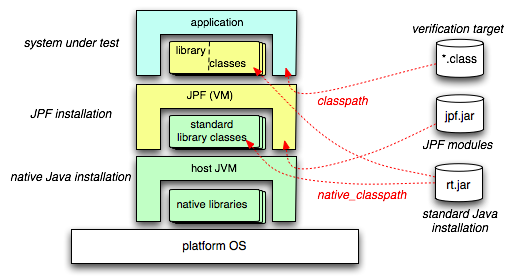
\includegraphics[scale=0.5]{images/layersJDart.png}
				\caption{\label{fig:jdart_layers} Les différents niveaux de l'environnement }
			\end{figure}
			
			De plus, combiner le framework JavaCard, \gls{JPF} et ses extensions ce qui demande des connaissances approfondies sur les propriétés des machines virtuelles
			Java et JavaCard, Pour pouvoir effectuer des testes en utilisant la technique d'éxécution concolique sur des applets JavaCard
			il est nécessaire de modifier l'API JavaCard à cause des méthodes natives qui ne peuvent pas être éxécuter sur JDart.
			Pour cela il faut intégrer la librairie JavaCard au sein de la machine virtuelle Java.
			
	\section{Tester des applets JavaCard}
		\paragraph{}
			Au cours de ce projet, nous essayerons de travailler sur tous les aspects et les fonctionalités d'une applet JavaCard.
			Pour exécuter des testes concoliques sur des applets il faut choisir les attribues à traiter comme variables concoliques et ceux
			qui doivent être traiter d'une maniére concrète.
			Dans la majorité des cas, on se contentera de traiter la classe APDU concoliquement puisque les requêtes passées à la méthode \verb|process()|
			de l'applet dépends de la valeur de la commande APDU.
	\section{Etendre les testes}
		\paragraph{}
			Exécuter \gls{JPF} sur le système sous test donne une vue claire sur la structure de l'applet à tester, de plus, nous voulons
			vérifier si l'applet est bien conforme à la spécification \textit{ISO 7816} et que toute transition d'un état à un autre est valide.
			La solution que nous proposons est d'utiliser la sortie de JDart pour générer un automate qui decrit tous les états et les transitions
			d'une applet.
			Puisque \gls{JPF} fait la vérification du modèle, concrètiser cette idée est relativement facile.
			En effet, nous détaillerons cette solution dans les chapitres suivants.
			
	\section{Interêt et limites}
	\paragraph{}
		\textbf{Java Path Finder} est connu comme le couteau suisse de la vérification Java,
		il est en effet un des outils de tests les plus évolués pour les applications Java,
		notamment grâce à son extensibilité et à son habilité à supporter et intérger de nouvelle extensions.
		Cependant, la majorité des extensions ne sont pas destinées à être executées sur des systèmes JavaCard ce qui nous a motivé
		à faire le choix de ce projet et à contribuer à la communauté.